\begin{section}{Basic Structures}{\label{sec1}}

In this section, the basic structures needed to understand hash-based signature algorithms will be explained.


\begin{subsection}{Hash Functions}

    Cryptographic hash functions are functions that convert input data of any length into a fixed-length digest value. In order for these functions to be used securely, they must satisfy certain fundamental properties. These properties are as follows:

    \begin{enumerate}[label=\textbf{\arabic*.}]
    \item \textbf{Collision Resistance}: The probability that two different inputs produce the same hash value must be very low. In other words, the condition \( h(x) = h(y) \) for \( x \neq y \) should be extremely rare. This property is one of the cornerstones of hash function security, and finding collisions should be computationally infeasible.

    \item \textbf{Pre-image Resistance}: It must be difficult to find the input that produces a given hash value. That is, given any hash output \( h(x) \), it should be computationally hard to find the corresponding input \( x \).

    \item \textbf{Second Pre-image Resistance}: Given a specific input and its hash value, it should be difficult to find a different input that produces the same hash value. In other words, given \( h(x) \), it should be computationally hard to find a different \( y \neq x \) such that \( h(y) = h(x) \).
    
    \end{enumerate}

Attack complexities of n-bit Hash function is given in Table \ref{tab:hash-complexities}

\begin{table}[h!]
  \centering
  \caption{Attack Complexities on an \(n\)‐bit Hash}
  \label{tab:hash-complexities}
  \begin{tabular}{|l|c|c|}
    \hline
    \textbf{Attack}            & \textbf{Classical Work} & \textbf{Quantum Work} \\ \hline
    Preimage                   & \(2^n\)                 & \(2^{n/2}\)           \\ \hline
    Second–Preimage            & \(2^n\)                 & \(2^{n/2}\)           \\ \hline
    Collision                  & \(2^{n/2}\)             & \(2^{n/3}\) (Brassard–Høyer–Tapp \cite{Brassard_1998}) \\ \hline
  \end{tabular}
\end{table}

\end{subsection}

\begin{subsection}{Lamport One-Time Signature}

\begin{figure}[h]
\centering
\begin{tikzpicture}[
    node distance=1.5cm and 2.5cm,
    secret/.style={rectangle, draw, rounded corners, fill=red!20, minimum height=1.5em, minimum width=4em, drop shadow},
    public/.style={rectangle, draw, rounded corners, fill=blue!20, minimum height=1.5em, minimum width=4em, drop shadow},
    msg/.style={rectangle, draw, fill=green!20, minimum height=1.5em, minimum width=2em},
    sig/.style={rectangle, draw, fill=orange!20, minimum height=1.5em, minimum width=4em, drop shadow},
    arrow/.style={-Latex, thick, draw=gray!80}
]
% Nodes for secret key
\node[secret] (sk00) {$sk_{i,0}$};
\node[secret, below=of sk00] (sk01) {$sk_{i,1}$};

% Nodes for public key
\node[public, right=of sk00] (pk00) {$pk_{i,0}$};
\node[public, right=of sk01] (pk01) {$pk_{i,1}$};

% Arrows from secret to public
\draw[arrow] (sk00) -- (pk00) node[midway, above] {$H$};
\draw[arrow] (sk01) -- (pk01) node[midway, above] {$H$};

% Labels for key pairs
\node[above=0.5cm of sk00, xshift=1.25cm] {\textbf{Secret Key}};
\node[above=0.5cm of pk00, xshift=1.25cm] {\textbf{Public Key}};

% Message and Signature part
\node[msg, below=3cm of sk00, xshift=1.25cm] (M) {$M_i=1$};
\node[sig, right=of M] (S) {$s_i = sk_{i,1}$};
\node[left=0.5cm of M] {\textbf{Message Bit:}};
\node[above=0.1cm of S] {\textbf{Signature Part}};

% Arrow showing selection
\draw[arrow, dashed, bend right=45] (M.north) to (sk01.south);
\draw[arrow, dashed, bend left=10] (sk01.east) to (S.west);

\end{tikzpicture}
\caption{Lamport Signature Scheme}

\end{figure}
The Lamport signature scheme \cite{lamport1979constructing} is the first known hash-based signature algorithm. This scheme generates signatures that can only be used once, hence requiring a different key pair for each message. The steps of the scheme are as follows:

\begin{subsubsection}{Lamport Key Generation}
    Let us assume that a 256-bit message will be signed. In the Lamport algorithm, each bit of the signature requires 2 keys, resulting in a total of 512 public and private keys. The private keys are generated randomly and grouped as follows:

    \[
    \text{sk}_0 = \text{sk}_{10}, \text{sk}_{20}, \ldots, \text{sk}_{2560}
    \]
    \[
    \text{sk}_1 = \text{sk}_{11}, \text{sk}_{21}, \ldots, \text{sk}_{2561}
    \]
    
    The public keys are obtained by applying a hash function to each private key:
    
    \[
    \text{pk}_0 = H(\text{sk}_{10}), H(\text{sk}_{20}), \ldots, H(\text{sk}_{2560})
    \]
    \[
    \text{pk}_1 = H(\text{sk}_{11}), H(\text{sk}_{21}), \ldots, H(\text{sk}_{2561}) \]
    
\end{subsubsection}

\begin{subsubsection}{Lamport Signature}

    Each bit of the message is examined. If the bit is 0, the corresponding part of the signature is taken from the \(\text{sk}_0\) group; if the bit is 1, it is taken from the \(\text{sk}_1\) group.

    For example, suppose the first three bits of our message are "001". Then, the first three parts of the signature would be:

    \[
    \text{sk}_{10} \| \text{sk}_{20} \| \text{sk}_{31}
    \]
    
\end{subsubsection}

\begin{subsubsection}{Signature Verification}

    The verifier examines each bit of the message one by one. If the bit value is 0, the hash of the corresponding part of the signature is computed and compared with the corresponding part of \(\text{pk}_0\). If the bit is 1, it is compared with the corresponding part of \(\text{pk}_1\).

    This process is repeated for all bits. If all comparisons are equal, then the signature is successfully verified.
    
\end{subsubsection}
    
\end{subsection}

\begin{subsection}{WOTS and WOTS+}

    The WOTS (Winternitz One-Time Signature) algorithm \cite{buchmann2013security}, like the Lamport signature algorithm, is a one-time signature scheme. While in the Lamport algorithm each bit of the message is signed individually, in the WOTS scheme the message is divided into chunks of \( w \) bits, and each chunk is signed instead of individual bits. 

    As a result, the signature size becomes \( w \) times smaller compared to the Lamport scheme. However, a \( w \)-bit message chunk can take \( 2^w \) different values, and a private key is required for each possible value.

    This problem is also addressed using hash functions.

    \begin{subsubsection}{WOTS Key generation}

        Let us assume that the message is divided into \( N \) parts, each consisting of \( l \) bits. In this case, \( N \) secret keys \( \text{sk}_0, \text{sk}_1, \ldots, \text{sk}_N \) are randomly generated. The \( 2^l \) possible values that each part can take are obtained by applying a hash function repeatedly to the randomly generated keys.

        \begin{figure}
            \centering
            \begin{tikzpicture}[
        node distance=0.8cm and 0.8cm,
        box/.style={
          draw,
          minimum width=1.5cm,
          minimum height=0.8cm,
          align=center
        },
        arr/.style={-{Latex}}
      ]

      % First row: sk_0 → h(sk_0) → h^2(sk_0) → … → h^{2^i−1}(sk_0)
      \node[box] (sk0)    {sk$_0$};
      \node[box,right=of sk0] (hsk0)  {h(sk$_0$)};
      \node[box,right=of hsk0] (h2sk0) {h$^2$(sk$_0$)};
      \node[right=of h2sk0]        (dots0) {$\cdots$};
      \node[box,right=of dots0]  (h2i1sk0) {h$^{2^l-1}$(sk$_0$)};
      \draw[arr] (sk0) -- (hsk0) -- (h2sk0) -- (dots0) -- (h2i1sk0);
    
      % Second row: sk_1 → h(sk_1) → h^2(sk_1) → … → h^{2^i−1}(sk_1)
      \node[box,below=of sk0]    (sk1)    {sk$_1$};
      \node[box,right=of sk1]    (hsk1)   {h(sk$_1$)};
      \node[box,right=of hsk1]   (h2sk1)  {h$^2$(sk$_1$)};
      \node[right=of h2sk1]      (dots1)  {$\cdots$};
      \node[box,right=of dots1] (h2i1sk1){h$^{2^{l-1}}$(sk$_1$)};
      \draw[arr] (sk1) -- (hsk1) -- (h2sk1) -- (dots1) -- (h2i1sk1);
    
      % Last row: sk_{N-1} → h(sk_{N-1}) → h^2(sk_{N-1}) → … → h^{2^i−1}(sk_{N-1})
      \node[box,below=of sk1]    (skN)    {sk$_{N-1}$};
      \node[box,right=of skN]    (hskN)   {h(sk$_{N-1}$)};
      \node[box,right=of hskN]   (h2skN)  {h$^2$(sk$_{N-1}$)};
      \node[right=of h2skN]      (dotsN)  {$\cdots$};
      \node[box,right=of dotsN] (h2i1skN){h$^{2^l-1}$(sk$_{N-1}$)};
      \draw[arr] (skN) -- (hskN) -- (h2skN) -- (dotsN) -- (h2i1skN);
    
        \end{tikzpicture}
            \caption{WOTS key generation}
            \label{fig:WOTS}
        \end{figure}

        In Figure \ref{fig:WOTS}, the secret keys are shown. The public key is obtained by applying the hash function \( 2^l \) times to each secret key (i.e., the \( 2^l \)-th hash). 

        For example, if the value of the first message chunk is 0, then \(\text{sk}_0\) is used in the signature. If the value is \( 2^l - 1 \), then the signature value is \( h^{2^l - 1}(\text{sk}_0) \).

        
    \end{subsubsection}

    \begin{subsubsection}{WOTS Signature}

        For each part of the message, the appropriate number of hash iterations is applied to the corresponding secret key. These hashed values are concatenated to form the complete signature.

        For example, suppose the first three chunks of the message are:
        
        \[
        001 \| 010 \| 111
        \]
        
        Then the first three parts of the signature would be:
        
        \[
        h(\text{sk}_0) \| h^2(\text{sk}_1) \| h^7(\text{sk}_2)
        \]
                
    \end{subsubsection}

    \begin{subsubsection}{WOTS Signature Verification}

        The verifier examines each message part individually. By checking the numerical value of each chunk, the verifier determines how many hash iterations are needed to reach the public key. It then hashes the corresponding part of the signature that many times. The result is compared with the known public key. If all values match, the signature is considered valid.
        
    \end{subsubsection}

    \begin{subsubsection}{WOTS+ \cite{cryptoeprint:2017/965}}

        Introduced as an improved variant of WOTS. The primary difference is that WOTS+ introduces a randomized bitmasking technique in its chaining function. Specifically, before each hash computation in the signature generation and verification process, WOTS+ XORs a randomly generated bitmask with the input. This masking mitigates multi-target attacks and improves the scheme’s resistance to attacks that exploit structural properties of the hash function. 
        
    \end{subsubsection}
    
    
\end{subsection}


\begin{subsection}{Merkle Trees and Multi-Signatures}

Lamport and WOTS schemes are one-time signature algorithms, meaning they allow signing only a single message with generated keys. However, in practical scenarios, signature algorithms are expected to support multiple signatures. To convert one-time signature schemes into algorithms that can sign multiple messages, \textbf{Merkle trees} are used.

As an example, the WOTS scheme can be used together with a Merkle tree. Figure \ref{fig:Merkle} shows the sketch of merkle tree used with WOTS. The bottom leaves of the Merkle tree are the hash values of the WOTS public keys. Using a Merkle tree of height \( h \), a signature scheme capable of signing \( 2^h \) messages can be constructed.

In addition to increasing signature capacity, Merkle trees also have the advantage of \textbf{reducing public key size}. Normally, a WOTS public key consists of multiple components—one for each message chunk—but when used with a Merkle tree, only \textbf{one public key} is required: the root of the Merkle tree.To verify a signature, the verifier must access certain intermediate nodes of the Merkle tree in order to compute the root. These intermediate values can be included as part of the signature, thus enabling successful verification.

\begin{figure}
    \centering
    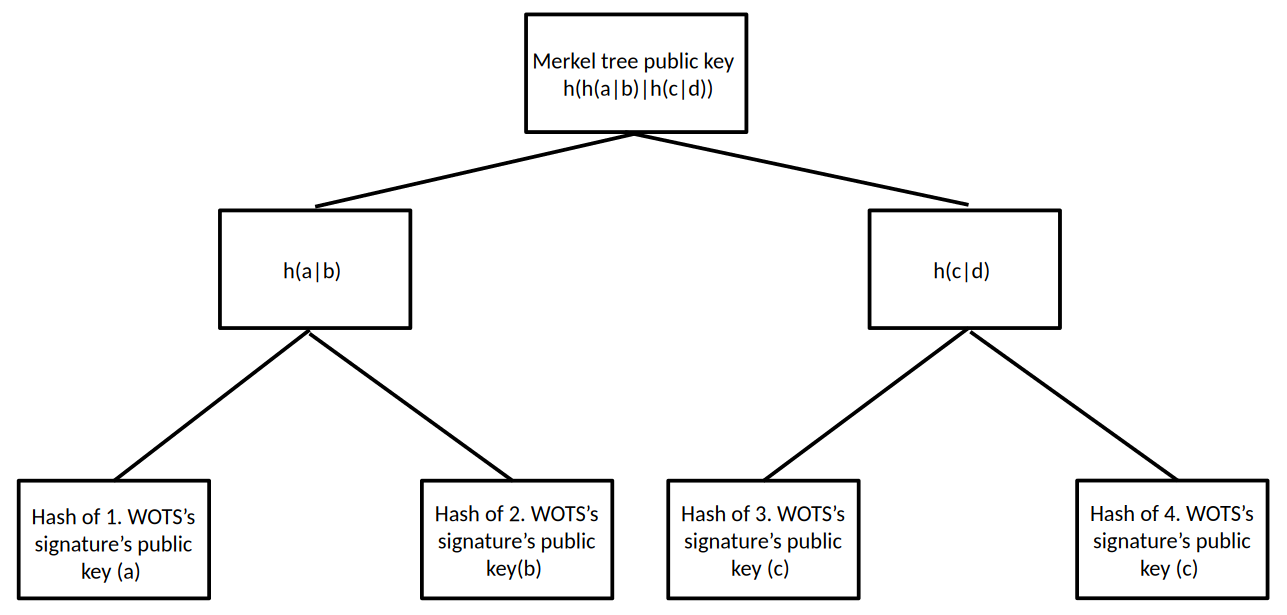
\includegraphics[width=1.1\linewidth]{fig/merkle.png}
    \caption{Merkle Tree}
    \label{fig:Merkle}
\end{figure}

\end{subsection}

\begin{subsection}{L-tree and Hashing public key}{\label{sec:L-tree}}

    When combining one-time signature schemes with a Merkle tree, the public key of the one-time signature scheme is selected as the bottom leaf of the Merkle tree. However, in the WOTS algorithm, a single signature includes not one but multiple public key components—one for each message part.
    
    To resolve this issue, two different approaches are employed:
    
    \begin{enumerate}
        \item \textbf{L-tree (used in XMSS):} The L-tree is a specialized Merkle tree used to compress multiple public key components into a single public key. It repeatedly hashes pairs of public key elements until only one remains.
    
        \item \textbf{Hashing (used in SPHINCS+):} In this method, all public key components are concatenated, and a single hash value is computed over the entire concatenation. This resulting hash serves as the single public key for Merkle tree integration.
    \end{enumerate}

    
\end{subsection}

\begin{subsection}{Base-\texorpdfstring{$w$}{w} Representation }

In hash-based signature schemes such as WOTS and XMSS, the message digest is first transformed into a base-$w$ representation before signing. This \textbf{base-$w$ representation} is a critical component of the signing process and directly influences the structure and security of the signature.

The main purposes of using base-$w$ representation are to:

\begin{itemize}
    \item reduce the size of the signature compared to bit-wise representations (as in the Lamport scheme),
    \item represent the message digest in a form suitable for the Winternitz one-time signature construction,
    \item control the number of hash iterations per key chain in WOTS+,
    \item and balance the trade-off between performance (speed) and signature length through the choice of $w$.
\end{itemize}

Let the output of the hash function be $n$ bits. The number of base-$w$ digits required to represent this $n$-bit message is:
\[
\ell_1 = \left\lceil \frac{8n}{\log_2 w} \right\rceil
\]
Each digit in this representation is an integer in the range $[0, w-1]$, and indicates how many times the corresponding chain of the private key should be hashed to produce the signature component.

\textbf{Example:}  
Suppose $n = 256$ and $w = 16$. Then:
\[
\ell_1 = \left\lceil \frac{8 \cdot 256}{\log_2 16} \right\rceil = \left\lceil \frac{2048}{4} \right\rceil = 512
\]
So, the hash output will be split into 512 base-$16$ digits.

After computing the base-$w$ representation of the message digest, a checksum is computed and appended (as described in the section \ref{sec:Checksum}), forming the complete message input for WOTS+.

The choice of $w$ is significant: 
\begin{itemize}
    \item A smaller $w$ increases the number of digits $\ell_1$ (and thus the signature size) but reduces the number of hash computations.
    \item A larger $w$ reduces the signature size but requires more hash computations per signature, increasing signing and verification time.
\end{itemize}

In summary, the base-$w$ representation enables the WOTS+ signature scheme to efficiently encode the message digest while maintaining flexibility across a range of parameter choices.

\end{subsection}


\begin{subsection}{Checksum}{\label{sec:Checksum}}

In hash-based signature algorithms such as WOTS and XMSS, the message to be signed is first encoded into a base-$w$ representation. However, this encoding alone is not sufficient to ensure security against certain attacks. Therefore, a \textbf{checksum} value is appended to the base-$w$ representation of the message. This checksum serves to:

\begin{itemize}
    \item prevent attacks that attempt to alter message chunks by increasing or decreasing hash iterations,
    \item protect against fault injection attacks that aim to exploit the absence or corruption of the checksum,
    \item and detect message modifications or signature reuse.
\end{itemize}

The checksum is calculated by summing the differences between the maximum possible chunk value $(w-1)$ and each base-$w$ digit of the message. If the message is represented by $m_0, m_1, \ldots, m_{\ell_1-1}$ in base-$w$, the checksum $c$ is given by:
\[
c = \sum_{i=0}^{\ell_1-1} (w - 1 - m_i)
\]
This value is then encoded into base-$w$ as an additional sequence of digits, forming the checksum part of the message. The total number of checksum digits required is $\ell_2$, calculated as:
\[
\ell_2 = \left\lfloor \frac{\log_2(\ell_1(w-1))}{\log_2 w} \right\rfloor + 1
\]

As a result, the full message to be signed by WOTS+ consists of $\ell = \ell_1 + \ell_2$ base-$w$ digits. Each digit corresponds to the number of hash function applications to be performed on a particular chain of the private key.

\textbf{The checksum} plays a crucial role in maintaining the integrity and one-time nature of the WOTS+ signature. Without it, an attacker could transform a valid signature for one message into a valid signature for another message by manipulating the hash chains, which would compromise the existential unforgeability of the scheme.

\end{subsection}


\begin{subsection}{FORS}
    The \textbf{FORS algorithm} (Forest of Random Subsets) is a \textit{few-time signature scheme}. Unlike the WOTS algorithm, in FORS, when the message is divided into parts, a secret key is generated for each possible value of every part, and a small Merkle tree is constructed from these keys.
    The signature consists of:
    \begin{itemize}
        \item The secret key corresponding to the integer value of the message part.
        \item The necessary authentication path (intermediate nodes) to reach the root of the Merkle tree.
    \end{itemize}
    An example FORS signature for the below message is shown in Figure \ref{fig:FORS}.
    
    \[100 \quad 011 \quad 011 \quad 101 \quad 111 \quad 000\]
    
    
    \begin{figure}
        \centering
        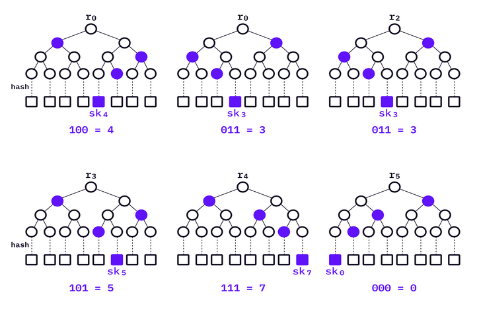
\includegraphics[width=0.9\linewidth]{fig/FORS.png}
        \caption{FORS Signature example }
        \label{fig:FORS}
    \end{figure}

\end{subsection}

\begin{subsection}{Address Structures in Hash-Based Signature Schemes}
    Hash-based signature schemes consist of either very large Merkle trees or multi-layered Merkle trees in order to increase their signature capacity. Since the same hash function is repeatedly used within the tree and similar operations are performed, \textbf{address structures} are used in hash-based signature schemes to:
\begin{itemize}
    \item distinguish each operation,
    \item determine the position within the tree,
    \item track how many hash operations have been applied,
    \item and provide input differentiation for the hash functions.
\end{itemize}

\textbf{Table} \ref{tab: Adress} shows the \textbf{OTS address structure} used in the XMSS algorithm \cite{huelsing2018rfc}. In the example structure, the following fields appear in order from top to bottom:
\begin{itemize}
    \item the layer in the multi-tree,
    \item the specific tree identifier,
    \item address type (e.g., OTS),
    \item index of the L-tree–WOTS pair,
    \item WOTS chain identifier,
    \item index of the hash operation within the chain,
    \item a flag indicating whether the hash value is used for encryption or masking.
\end{itemize}

Depending on the algorithm and its internal structure, the format of the address field can vary.


\begin{table}[H]
\centering
\renewcommand{\arraystretch}{1.5}
\begin{tabular}{|c|c|}
\hline
\textbf{Field} & \textbf{Size} \\
\hline
layer address     & 32 bits \\
\hline
tree address      & 64 bits \\
\hline
type = 0          & 32 bits \\
\hline
OTS address       & 32 bits \\
\hline
chain address     & 32 bits \\
\hline
hash address      & 32 bits \\
\hline
keyAndMask        & 32 bits \\
\hline
\end{tabular}
\caption{XMSS OTS Address Format}
\label{tab: Adress}
\end{table}

\end{subsection}

\begin{subsection}{Stateful and Stateless Hash-Based Signature Schemes}

    Hash-based signature algorithms can be categorized into two types: \textbf{stateful} and \textbf{stateless}. The fundamental difference between these two categories lies in the management of state information during the signature generation and verification processes.

\textbf{Stateful hash-based signature algorithms} require the maintenance of state information while generating signatures. These algorithms rely on \textit{one-time keys} that can be used only once per signature operation. Reusing these keys leads to serious security vulnerabilities. A representative example of such an algorithm is XMSS \cite{huelsing2018rfc}.

\textbf{Stateless hash-based signature algorithms}, in contrast, do not require any state information to be stored during the signing process. A prominent example of a stateless algorithm is SPHINCS+ \cite{bernstein2019sphincs+}.
    
\end{subsection}

\end{section}